\documentclass[__main__.tex]{subfiles}
\begin{document}
	
	\qtitle{Ч}{11}
	Электрон в сферически симметричном потенциале. Главное, орбитальное, магнитное квантовые числа. Опыт Штерна-Герлаха. Гипотеза спина электрона.\\ 
	
\textbf{Электрон в сферически симметричном потенциале. Главное, орбитальное, магнитное квантовые числа.}
Рассматривая стационарное уравнение Шредингера для электрона в сферически симметричном потенциале разделяя радиальную и угловую переменные мы придем к выводу, что уравнению Шредингера удовлетворяют собственные функции , которые определяются 3-я квантовыми числами:
\begin{itemize}
	\item $n$ - главное квантовое число, определяет номер орбиты, т.е энергетические уровни электрона в атоме
	\begin{gather*}
		n = 1,2,3,\cdots
	\end{gather*}
	\item $l$ - орбитальное квантовое число определяет момент импульса электрона в атоме
	\begin{gather*}
		l = \underbrace{0,1,2,\cdots,n-1}_{\text{$n$ - значений}}
	\end{gather*}
	\item $m_l$ - магнитное квантовое число определяет проекцию момента импульса электрона на заданное направление (направление внешнего магнитного поля) – пространственное квантование.
	\begin{gather*}
		m_l = \underbrace{0,\pm1,\pm2,\cdots,\pm l}_{\text{$2l+1$ - значений}}
	\end{gather*}
\end{itemize}


\textbf{Опыт Штерна-Герлаха}\\
На атом обладающий магнитным моментом $\vec{\mu}$, в неоднородном магнитном поле $\vec{B}$ должна действовать сила
\begin{gather*}
	\vec{f} = \left(\vec{\mu}\cdot\nabla\right)\vec{B}
\end{gather*}
Чтоб рассуждать было проще, пусть $B_x, B_y = 0$  и $B_z \neq 0$, тогда
\begin{gather*}
	\vec{f} = \left(\mu_x\partial_xB_z+\mu_y\partial_yB_z+\mu_z\partial_zB_z\right)\vec{e}_z
\end{gather*}
направлена либо по либо против $z$. Пусть неоднородность создана лишь вдоль $z$ тогда $\partial_xB_z=0; \partial_yB_z=0$\\\\
Опыт выглядит довольно просто: направим пучок атомов в область неоднородного магнитного поля и посмотрим что будет на выходе из этой области.
%probably will be useful to put image
В области неоднородного магнитного поля на атомы с $\mu_z \neq 0$ действует сила $f_z \sim \mu_z$; в результате они отклоняются от первоначального направления; величина отклонения тем больше, чем больше $|\mu_z|$; вверх или вниз зависит от знака $\mu_z$.
Согласно квантовой механике $\mu_z$ квантуется $\Rightarrow$ исходный пучок обязан расщепиться на число пучков, равное числу разрешенных $\mu_z$. В итоге должно получится что-то вроде(\textbf{пространственное квантование} -- набор эквидистантных пятен на экране):
\newpage
\begin{figure}[h]
	\center{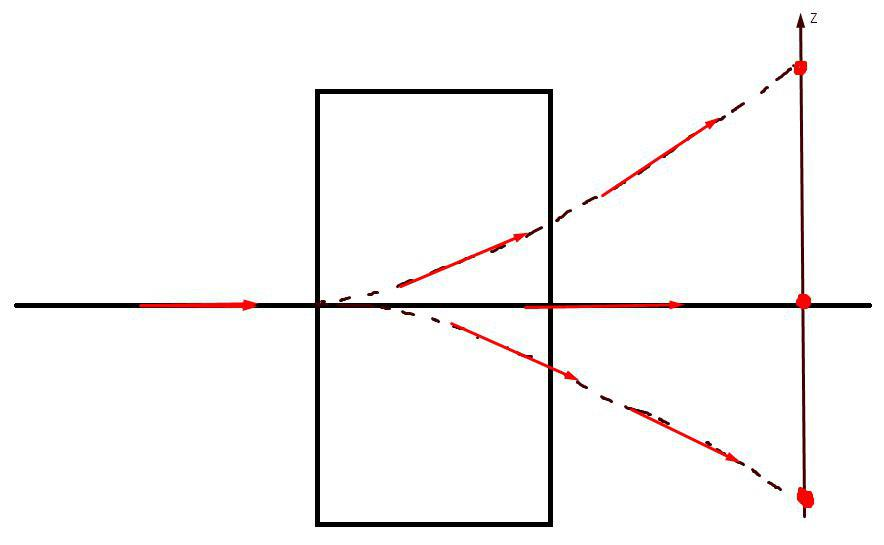
\includegraphics[width=0.9\linewidth]{ch-18}}
\end{figure}

\textbf{Гипотеза спина электрона}\\
Подсчитаем число пучков на выходе из неоднородного $\vec{B}$. Вопрос: Сколько возможных $\mu_z$ ?
\begin{gather*}
	\mu_z = -\mu_Bm
\end{gather*}
где $\mu_B$ - магнетон Бора.\\
При фиксированном $l$ число возможных $m$ составляет $2l+1$ и учитывая, что $l,n \in N$, приходим к выводу, что число возможных $m$ - нечетное. Проверим это:\\
Для этого пропустим пучок атомов водорода с $l=0$ через область неоднородного магнитного поля. Поскольку $l = 0 \Rightarrow m = 0 \Rightarrow \mu_z = 0 \Rightarrow$ пучок должен проследовать прямо в центр экрана, НО это не так - он расщепляется на две составляющие! Таким образом приходиться предположить, что электрон обладает собственным моментом импульса или спином, которому соответствует некоторый магнитный момент. Приходим к определению полного момента импульса частицы:
\begin{gather*}
	\hat{J} = \hat{L}+\hat{S}
\end{gather*} 
где $\hat{L}$ - орбитальный момент, $\hat{S}$ - спин.\\\\
Ввиду того (как оказалось), что электрон обладает внутренней степенью свободы(спином), то теперь для того, чтобы охарактеризовать его стационарные состояния в поле ядра нам потребуется уже не 3 квантовых числа а четыре (добавляется спиновое квантовое число - $m_s$)
	
\end{document}